\chapter{\LaTeX: Making Beautiful Documents}\label{ch:latex}
40 pages

\section{Why \LaTeX?}
\index{latex}
\index{WYSIWYG}
Most people need to write text documents from time to time, be it a CV, an article or a school assignment. Especially if you're writing something you'll use in your profession, you likely want it to \emph{look} professional which usually is not the case when you use tools like Microsoft Word or LibreOffice Writer. With these what-you-see-is-what-you-get (WYSIWYG) tools, the author spends time manually tweaking how stuff looks; where the title is, which fonts to use, text sizes, and placement. Most of us are not interested enough in typography to do this right. In comparison, using \LaTeX{}, the writer focuses on what stuff \emph{is}, rather than how stuff \emph{looks}. By telling \LaTeX{} ``this is a title'', or ``this is a new paragraph'' \LaTeX{} itself will figure out the proper formatting. It may seem unfamiliar at first that \LaTeX{} decides how stuff looks, indeed many novices try to force \LaTeX{} to display stuff in a particular way. My advice: don't!

\LaTeX{} certainly comes with a higher learning barrier before you can use it than WYSIWYG tools, but once you get familiar with it, I think you'll find that using it actually isn't that much slower, and it produces much better results. You may find a shift in what you spend time on: less time manually placing stuff, more time looking for how to do ``this thing'' with \LaTeX{} on the internet.

Other professional typesetting tools exist as well, but \LaTeX{} is very well developed and by far the most widespread, at least in scientific publications and books. We'll also see how to use it for making slideshow presentations, thus replacing tools such as Microsoft PowerPoint. If there's one typesetting tool you want in your toolbox to it's definitely \LaTeX{}.

\section{Which tools you need}
\index{highlighting}
\index{Texmaker}
\LaTeX{} can be written in any plain text editor (like Notepad if you're using Windows) and stored to a file ending with .tex. The .tex file is then \emph{compiled} to generate a .pdf-file using the command line tool \verb|pdflatex|. However, most users prefer a more specialized text editor which runs \verb|pdflatex| for you. Most such editors also supports highlighting, i.e.\ the application of different colors to different parts of the code to make it more readable. Many good editors exist, but we will use Texmaker which works on both Linux, OS X and Windows.

To get \LaTeX{}, you need to install a \LaTeX{}-distribution on your computer. There are several of them, but the code you write is the same for all of them. Proceed according to your operating system to install a \LaTeX-distribution and Texmaker.

\subsection{Linux}
\index{TeX Live}
On Linux, TeX Live is the recommended distribution. On Ubuntu, Mint or Debian Linux, you can install TeX Live and Texmaker using the following command:
\begin{verbatim}
$ sudo apt-get install texlive-full texmaker
\end{verbatim}

\subsection{OS X}
\index{MacTeX}
For OS X, MacTeX is the recommended distribution. It is the essentially the same as TeX Live but adds some compatibility to OS X. Download and install MacTeX and Texmaker from the following links:

\begin{verbatim}
http://tug.org/mactex
http://www.xm1math.net/texmaker
\end{verbatim}

\subsection{Windows}
\index{MiKTeX}
For Windows either TeX Live or MiKTeX can be used, but many find MiKTeX slightly easier to handle. Install MiKTeX and Texmaker from the following links:

\begin{verbatim}
http://www.miktex.org
http://www.xm1math.net/texmaker
\end{verbatim}

\section{Our first document}
We will start by going through \reflst{latex:minimal} which is about the minimum code required to start a new document. The left part is the source code while the right part demonstrates the output produced by the code. The actual result will necessarily be slightly different, since it will be placed in its own document with its own page, margins and formatting, but a demonstration may be instructive in some case nonetheless.

\begin{listing}
	\rule{\textwidth}{0.4pt}
	\begin{minipage}[t]{0.49\textwidth}
		\inputminted[frame=none]{latex}{latex/first.tex}
	\end{minipage}\hfill\vline\hfill
	\begin{minipage}[t]{0.49\textwidth}
		Here is some text.
	\end{minipage}\\[0.5em]
	\rule{\textwidth}{0.4pt}
	\caption{A (near-)minimal \LaTeX{} document}
	\label{lst:latex:minimal}
\end{listing}

\index{command}
\index{argument}
\index{option}
Notice that all \LaTeX{}-\emph{commands} start with a backslash, and may be followed by mandatory \emph{arguments} in curly braces, and optional arguments (\emph{options}) in square brackets like this:

\index{syntax}
\latexone|\command[option1,option2]{argument1}{argument2}|
\noindent Such ``rules'' for how commands are structured is usually referred to as \emph{syntax}.

\index{\latexin{\documentclass}}
The first command in any document is \latexin{\documentclass} which tells \LaTeX{} what kind of document it is. Some possible arguments are shown in \reftab{latex:documentclass}. The option \latexin{a4paper} tells \LaTeX{} to produce a document in paper size A4. \latexin{\documentclass} also support options for other paper sizes, font sizes, etc.\ which you can find on the internet whenever you need it.

\begin{table}
	\centering
	\caption{Document classes}
	\begin{tabular}{ll}
	\hline
	\latexin{book}		&	For books.																\\
	\latexin{report}		&	For reports and somewhat big documents (tens of pages).					\\
	\latexin{article}	&	For articles and smaller documents. Excludes chapters.					\\
	\latexin{beamer}		&	For	slideshow presentations using the Beamer package.						\\
	\latexin{curve}		&	For CVs using the Curve package.
	\end{tabular}
	\label{tab:latex:documentclass}
\end{table}

\index{\latexin{\usepackage}}
\index{\latexin{inputenc}}
\index{\latexin{fontenc}}
\index{\latexin{babel}}
\index{package}
\index{font encoding}
\index{character encoding}
Next, the functionality of \LaTeX{} can be expanded by including \emph{packages} which provides more features (similar to \emph{modules} in Python or \emph{libraries} in other languages). This is done by the \mintinline{latex}{\usepackage} command, one per package you want to use. To begin with, we need three packages: \latexin{inputenc} specifies the \emph{character encoding} which is used in the .tex files. We'll get back to this. \mintinline{latex}{fontenc} determines the \emph{font encoding} to be used in the .pdf-file. We won't dig into this but it should usually be T1. Finally, \mintinline{latex}{babel} specifies the written language.

\index{environment}
\index{\latexin{\begin}}
\index{\latexin{\end}}
\index{comment}
%The next new thing we'll encounter is an \emph{environment}. An environment starts with a \latexin{\begin} and ends with an \latexin{\end}, and affects anything in between. The \latexin{document} environment is where you write what actually goes into the document. Everything before it, is called the \emph{preamble} and is not actually printed to the document. Here we only have the text ``Here is some text.'' and a \emph{comment}, which is text \LaTeX{} completely ignores. Everything following a \% is a comment. Comments are only for your own convenience; you may write comments for instance about what commands does, why you chose to write something the way you did, etc.
The next new thing we'll encounter is an \emph{environment}. An environment starts with a \latexin{\begin} and ends with an \latexin{\end}, and affects anything in between. The \latexin{document} environment is where you write what actually goes into the document. Here, the only thing in the document is the text ``Here is some text.''. Text is written straight forward, with a few exceptions which we'll get back to. When \LaTeX{} encounters a \% character, it ignores anything on the rest of that line. This is known as a \emph{comment} and is only visible in the source code. You may use comments to explain things which is not obvious in the source code for later reference.

\index{preamble}
The part between \latexin{\documentclass} and \latexin{\begin{document}} which is used to load packages, and make other configurations to the document is known as the \emph{preamble}.

\subsection{Character Encoding}
\index{character encoding}
\index{ASCII}
\index{UTF-8}
Whenever text is stored in a file it is represented by strings of zeros and ones (\emph{binary digits} or just \emph{bits}) according to a \emph{character encoding standard}. An early standard is the \emph{ASCII} standard (American Standard Code for Information Interchange) which uses 7 bits to represent letters. For instance, ``A'' is represented by the binary number 1000001 which maps to 65 when converted to the decimal system. Since 7 bits can only encode 128 characters, only the most common characters were included in the ASCII standard. By expanding it with one bit, 128 characters more could be encoded. However, this is still not enough for all kinds of languages, and as a result, different 8 bit encodings exist depending on where you're from. One of the most popular is ISO-8859-1 which includes the letters used in Western European languages. However, then you cannot use letters outside of this standard. UTF-8, on the other hand, is a very clever encoding which circumvents this problem by using 8 bits (or one byte) for the most common characters but may use up to four bytes for rarer characters. As such, UTF-8 has a wide range of characters and should cover all your needs while not making the text documents much larger. I recommended storing all .tex files as UTF-8 to avoid encoding problems.

In Texmaker you can ensure files are stored as UTF-8 by going to Options$\rightarrow$ Configure Texmaker (see \reffig{latex:texmaker}), open the ``Editor'' pane and make sure ``Editor Font Encoding'' is set to UTF-8. Finally, the \LaTeX{} compiler needs to know the encoding to decode it correctly as well. This is what we've told it in the option for the \latexin{inputenc} package in \reflst{latex:minimal}. A common pitfall is that the \latexin{inputenc} option does not match the actual encoding used in the file which causes local/special (non-ASCII) characters to look like other symbols.

\begin{figure}
	\centering
	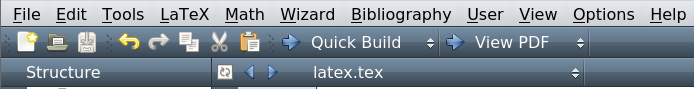
\includegraphics[width=\textwidth]{graphics/texmaker.png}
	\caption{Texmaker toolbar}
	\label{fig:latex:texmaker}
\end{figure}

\subsection{Compiling}
\index{compilation}
\index{\verb|latex|}
\index{\verb|pdflatex|}
The next step is to compile our minimal example to turn it into a .pdf file. The minimal example from \reflst{latex:minimal} can be saved to a UTF-8 encoded file \texttt{main.tex} in a new folder. You \emph{do} want to create a separate folder for each document you write since \LaTeX{} generates lots of other files in this folder upon compilation.

One should be aware that people use different compilation strategies. Some people use the program \texttt{latex} which generates a .dvi file and then converts it to .pdf using a conversion tool, while we will use the program \texttt{pdflatex} which directly generates the .pdf file. Both of these are command line programs but Texmaker can run these commands so we don't have to. However, to better grasp what's going on behind the curtains, we will see how it's done both from the command line and from Texmaker. If you haven't read \refch{bash} yet, don't worry. You don't need to be able to run the commands to proceed this chapter.

\subsubsection{Using the command line}
To compile \texttt{main.tex} using the (Linux, OS X or Windows) command line, navigate to the folder where the file is, and simply run:
\begin{verbatim}
$ pdflatex main.tex
\end{verbatim}
and a file named \verb|main.pdf| will be created. If you got no errors you're done.

But computers are very literal and errors is the most common thing. If there's a typo somewhere in your code, e.g. a capital letter instead of a small one in a command, the document simply will not compile, but returns an error. The error messages may look cryptic at first, but they do tell what the error is and which line it is on. You can exit the failed compilation in the command line by typing ``x''. Try to sort out one error at a time, starting with the top one.

Sometimes, when you have an error in your code, and you can't figure out what it is, it may be useful to \emph{comment out} a block of lines. Texmaker supports commenting out multiple lines by marking them and hitting Ctrl+T. Uncommenting the marked lines is done by Ctrl+U. Another advice: Compile your document often to avoid a bunch of errors to accumulate. Fixing errors is perhaps the largest barrier when starting to program, but it gets a lot easier with a little experience.

\subsubsection{Using Texmaker}
Next: compile using Texmaker. We can use the arrow next to the ``Quick Build'' drop down menu (see \reffig{latex:texmaker}) to run any of the programs available from the drop down menu. As an example, we can choose ``PDFLaTeX'' and click the arrow, and to view it, we can click the arrow next to ``View PDF''. The ``Quick Build'' option is useful, since it can be configured to run a series of commands in sequence. If you again go to Options$\rightarrow$Configure Texmaker and select the ``Quick Build'' pane you can set Quick Build to ``PdfLaTeX + View PDF''. In the ``Commands'' pane, you can see exactly which commands Texmaker uses when running this programs. These are fine as they are. Now, when you choose ``Quick Build'' and click the arrow, the document will be compiled and displayed. Like when using the command line errors must be resolved to make the document compile.

You are advised to successfully compile \reflst{latex:minimal} before proceeding, and to keep experimenting with what you learn as you go.

\section{Writing Text}
\index{reserved characters}
As previously mentioned, writing text in \LaTeX{} is \emph{mostly} straight forward, but there are some things you need to pay attention to. First up are the \emph{reserved characters} listed in \reftab{latex:reserved}. These characters have special meanings i \LaTeX{}, for instance ``\%'' starts a comment, and must therefore be written using a command. Consider this example:

\latexone{We offer a mortgage at 5% interest.}
\noindent Here the last character printed is ``5'' since the rest is a comment. The proper way to write this would be:

\latexone{We offer a mortgage at 5\% interest.}
\noindent This also illustrates how highlighting 

\begin{table}
	\centering
	\caption{Reserved Characters}
	\begin{tabular}{ll}
	\hline
	\latexin{\#}					&	\# 		\\
	\latexin{\$}					&	\$		\\
	\latexin{\%}					&	\%		\\	
	\latexin{\&}					&	\&		\\
	\latexin{\_}					&	\_		\\
	\latexin|\{|					&	\{		\\
	\latexin|\}|					&	\}		\\
	\latexin{\^{}}				&	\^{}		\\
	\latexin{\~{}}				&	\~{}		\\
	\latexin{\textbackslash{}}	&	\textbackslash
	\end{tabular}
	\label{tab:latex:reserved}
\end{table}

Next, quotations are written starting with two backticks and ending with two apostrophes:

\latexone{``What's up?'' said George.}
\noindent The backticks and apostrophes will be replaced by proper quotation marks. Just using \latexin{"} is incorrect. If you need nested quotations, use a single backtick and apostrophe for the inner quote:

\latexone{``George asked me `what's up'.''}
\noindent This will evaluate to:

\begin{quote}
``George asked me `what's up'.''
\end{quote}

\index{hyphen}
\index{en-dash}
\index{em-dash}
\index{minus}
Next, let's learn to distinguish between hyphens and different kinds of dashes. \emph{Hyphens} are used for joining words. \emph{En-dash} is used when talking about numbers in a range, e.g.\ the years 1980--1990, and \emph{em-dash} is used as punctuation --- for instance like this --- in a sentence.  See \reftab{latex:dashes}. Hyphens and dashes should not be used for ``minus''. Minus is written using math mode (\refsec{latex:equations}).

\begin{table}
	\centering
	\caption{Hyphen, dashes and minus}
	\begin{tabular}{llll}
	\hline
	Hyphen	&	\latexin{mother-in-law}			&	mother-in-law							\\
	En-dash	&	\latexin{pages 3--7}			&	pages 3--7								\\
	Em-dash	&	\latexin{``Let's see --- 15 euros''}		&	``Let's see --- 15 euros''		\\
	Minus	&	\latexin{The answer is $-4$}		&	The answer is $-4$
	\end{tabular}
	\label{tab:latex:dashes}
\end{table}

To emphasize part of a text use the command \latexin{\emph}, for instance:

\latexone{This is \emph{very} important!}
\noindent which becomes

\begin{quote}
	This is \emph{very} important!
\end{quote}

Emphasized text normally appear italic, that is, slanted and with more calligraphy-styled letters. You can also directly specify that text should be for instance \underline{underlined}, using commands from \reftab{latex:formatting}. However, you normally should not do that. Remember, you tell \LaTeX{} what stuff \emph{is} and \LaTeX{} takes care of how stuff \emph{looks}. And in my opinion, italic is the only thing that actually looks good. Just look at how the \underline{underlined} words on this page damages the aesthetics of the whole page! You don't need to notice that a word is emphasized until you're actually reading it.

Furthermore, what if you want to emphasize a word inside something that's for some reason already italic? \latexin{\emph} takes care of redefining the emphasized style appropriately, in this case it becomes roman (which is the default style):

\begin{quote}
\textit{This is \emph{very} important!}
\end{quote}

%While you \emph{can} tell \LaTeX{} to make text \textbf{bold} or \underline{underlined} text this is usually not what you want. Remember, you tell \LaTeX{} what stuff \emph{is} and \LaTeX{} takes care of how stuff \emph{looks}. Unless you want to interfere with how stuff looks, you really just want to tell \LaTeX{} to \emph{emphasize} something and let \LaTeX{} take care of how. The appropriate command to emphasize text, therefore, is \latexin{\emph}, which usually is equivalent to making text appear \textit{italic}, but not always. \emph{Consider for instance that you want to emphasize a \emph{single} word inside an emphasized sentence!} Some commands for formatting text is given in \reftab{latex:formatting}.

\begin{table}
	\centering
	\caption{Formatting}
	\begin{tabular}{ll}
	\hline
	\latexin{\textrm{Roman}}			&	\textrm{Roman}		\\
	\latexin{\textbf{Bold}}			&	\textbf{Bold}		\\
	\latexin{\textsl{Slanted}}		&	\textsl{Slanted}		\\	
	\latexin{\textit{Italic}}		&	\textit{Italic}		\\
	\latexin{\textsc{Small Caps}}		&	\textsc{Small Caps}	\\
	\latexin{\textsf{Sans Serif}}		&	\textsf{Sans Serif}	\\
	\latexin{\texttt{Teletype}}		&	\texttt{Teletype}	\\
	\latexin{\underline{Underlined}}	&	\underline{Underlined}
	\end{tabular}
	\label{tab:latex:formatting}
\end{table}

%\section{Formatting Old}
%Basically, \LaTeX{} takes care of formatting, but sometimes you may want to tell \LaTeX{} to emphasize a word. This is done using \latexin{\emph}. You generally do not tell \LaTeX{} to display text as bold, italic or underlined like in WYSIWYG programs, but rather to emphasize it. Then it is up to \LaTeX{} to emphasize it in the proper way (which normally is italic).
%
%Comments are written using two backticks in the beginning of the quote, and two single quote marks at the end like this:
%
%\latexone{``This is a quote''}
%
%The reason for not just using a normal double quote mark is that various languages have different conventions of how quotation marks looks like, e.g. <<quote>>, ,,quote'' or "quote". When using two backticks and two single-quote marks, \LaTeX{} replaces them by the proper quotation marks for your language.
%
%What do you think the command \latexin{\LaTeX{}} on line 18 in \reflst{latex:structure} do?
%
%In \reflst{latex:structure} we have also used the command \latexin{\lipsum}. This is a command which fills the document by some rather arbitrary sample text at this spot known as Lorem ipsum. Lorem ipsum is a piece of gibberish latin text which is commonly inserted into a document or web page before you have any actual contents just to get a feel for how it will look. \latexin{\lipsum}, however, is not provided by \LaTeX{} as-is but is rather provided to us by a package \latexin{lipsum}. To use \latexin{\lipsum}, we need to include this package in the preamble of our document (line 5 in \reflst{latex:structure}). The \LaTeX{}-distributions comes pre-loaded with a bunch of packages (especially TeX Live) so you will likely have most of them. If not, you'll need to install it separately.
%
%Make sure you understand each line in \reflst{latex:structure}. 
%
%\subsection{To put somewhere}
%In \reflst{latex:structure} we have also used the command \latexin{\lipsum}. This is a command which fills the document by some rather arbitrary sample text at this spot known as Lorem ipsum. Lorem ipsum is a piece of gibberish latin text which is commonly inserted into a document or web page before you have any actual contents just to get a feel for how it will look. \latexin{\lipsum}, however, is not provided by \LaTeX{} as-is but is rather provided to us by a package \latexin{lipsum}. To use \latexin{\lipsum}, we need to include this package in the preamble of our document (line 5 in \reflst{latex:structure}). The \LaTeX{}-distributions comes pre-loaded with a bunch of packages (especially TeX Live) so you will likely have most of them. If not, you'll need to install it separately.

\section{Document Structure}
\index{\latexin{\chapter}}
\index{\latexin{\section}}
\index{\latexin{\subsection}}
\index{\latexin{\subsubsection}}
A new chapter is started using the \latexin{\chapter} command, with the name of the chapter as its argument. Chapters can be split into \emph{sections} using the \latexin{\section} command, which again can be split into \emph{subsections} (\latexin{\subsection}) and further on to \emph{subsubsection} (\latexin{\subsubsection}). See \reflst{latex:structure} for an example. Numbering of chapters, sections and so on happen automatically.

%When we're writing a document, we likely want to structure it by splitting it into chapters. Chapters can again be split into sections, which again can be split into subsections and further on to subsubsections. The corresponding commands are, intuitively, \latexin{\chapter}, \latexin{\section}, \latexin{\subsection} and \latexin{\subsubsection}. You can see how these are used in \reflst{latex:structure} to structure the document. Numbering of chapters, sections and so on happen automatically.

\begin{listing}[H]
	\inputminted{latex}{latex/structure.tex}
	\caption{A \LaTeX{} document with some structure and text}
	\label{lst:latex:structure}
\end{listing}

A chapter is a rather big, voluminous entity. The chapter's title may well consume approximately half a page, like in this book. In smaller documents like articles, school assignments, etc., which may only be a few pages long, this is not appropriate. The  \latexin{article} document class is suitable in such cases since it does not have chapters. There, sections are the highest structural level.

Further on, \LaTeX{} do not care if you write a whole paragraph in one line, or split it up into more lines. It will not break the lines where you do, but where it deems appropriate. Different paragraphs are separated by an open line (line 25 in \reflst{latex:structure}). 

\subsection{Table of contents}
\index{\latexin{\tableofcontents}}
Due to \LaTeX{}'s awareness of contents, it can also auto-generate a table of contents for you. This is done with the \latexin{\tableofcontents} command on line 8. When compiling the document, \LaTeX{} makes a list of all the chapters and sections and then stores it in a file. Upon next compilation, when it encounters \latexin{\tableofcontents}, this list will be used to make the table of contents. Unfortunately, if you did any changes to the ordering of the chapters in between, this list is now outdated, and the table of contents is incorrect. This behavior is typical for \LaTeX{}, which stores auxiliary information in files after compilation. To remedy this, compile the document again.

\subsection{Dividing documents into several files}
As your document gets bigger, your \verb|main.tex| file may start looking like a mess and you just can't find the parts your looking for. In such cases, it is very useful to split the document into multiple files, for instance one file per chapter, section or any other appropriately sized chunks of text. Another benefit of this is that it gets easier to collaborate with others on the document. For instance, if you and your friend work on separate chapters, you can work on separate files.

\begin{listing}
	\inputminted{latex}{latex/multifiles.tex}
	\caption{A .tex file with chapters in separate subfiles}
	\label{lst:latex:multifiles}
\end{listing}

\reflst{latex:multifiles} shows a new \verb|main.tex| file which uses the \latexin{\input} command to load the contents of other files. If you use \latexin{\chapter{Introduction}
Programmers, engineers, scientists and tech-savvy people in general have had the opportunity to learn a bunch of different computer programs and programming languages which makes their everyday work in front of the computer both easier and more efficient. In comparison, less technically oriented people, who lack such a toolbox, often end up using inconvenient tools and therefore end up using inefficient and impractical solutions.

Consider for instance that you have hundreds of photos and you’d like to change the resolution on all of them? Or maybe add a watermark before sharing them? Or change the filename to include the date? Such tasks can be tedious if you don’t know the right tools. However, the file names of all files can be changed using a single command in the Bash command line interface. A script that adds a watermark to every image takes less then 20 lines of code using the Python scripting language. Of course, programming takes time to learn, and it’s not for everybody to become a full time professional programmer. But with the emergence of modern low-threshold scripting languages like Python, why should such handy techniques still be reserved for geeks only?

Another thing which many may benefit from is learning a professional typesetting tool like LaTeX to write documents. Applications, CV’s, reports, slideshows, etc. Because let’s admit it: Most of us aren’t typographists. We don’t know exactly which font to use, which size, which line spacing and which margins to use everywhere to make a document look professional. LaTeX takes care of all that for you, but then you need to tell LaTeX what’s supposed to be a chapter, what’s a new paragraph, and so on. And that’s done by coding. It doesn’t have to be that hard, to start a new chapter with the title “Introduction”, for instance, you simply type 

\latexone{\chapter{Introduction}}
And how do you generate a table of contents in LaTeX? Simple. Because LaTeX know what the chapters are, all you have to do is type:
\latexone{\tableofcontents}
where you want your table of contents.

And as a last example, have you ever had to collaborate with someone to write a document in a normal text processing tool such as Microsoft Word? Then you’ll know it’s a mess. No two people can edit the document at once, despite editing different parts of the file. Documents written in LaTeX, as well as programs written in languages such as Python can be efficiently shared amongs many users using a Version Control System (VCS) such as Git and everyone can work on it simultaneously without stepping on each other’s toes! VCSs like Git also allows you to backtrack the whole history of your documents in case you regret something you once did.

The aim of this little book is to provide the normal guy on the street with at least a small toolbox allowing him or her to work more efficiently. More in a similar manner as professionals. The tools presented are carefully selected because together, they form a minimal toolbox allowing the reader to use a computer in such a rich way. Moreover, they are considered to be more useful, versatile and simple to learn than other alternatives. Admittedly, we will only scratch the surface of all these tools. Just enough to get you started, with pointers of where to look for further information. True, it will not even cover the same depth as most beginner’s books, since it is not the aim of this book to turn you into a programmer. However, it is assumed that the reader, being a generation which has grown up with technology, is capable of finding his/her way around in simple graphical computer programs. Therefore this book will focus on the coding aspects, only providing pointers to which graphical programs may be useful (for instance to make figures in documents).

Finally, each part are self-contained and may be read independently of the other parts (although using Git is kind of meaningless without knowing some other coding).} or simply \latexin{\chapter{Introduction}
Programmers, engineers, scientists and tech-savvy people in general have had the opportunity to learn a bunch of different computer programs and programming languages which makes their everyday work in front of the computer both easier and more efficient. In comparison, less technically oriented people, who lack such a toolbox, often end up using inconvenient tools and therefore end up using inefficient and impractical solutions.

Consider for instance that you have hundreds of photos and you’d like to change the resolution on all of them? Or maybe add a watermark before sharing them? Or change the filename to include the date? Such tasks can be tedious if you don’t know the right tools. However, the file names of all files can be changed using a single command in the Bash command line interface. A script that adds a watermark to every image takes less then 20 lines of code using the Python scripting language. Of course, programming takes time to learn, and it’s not for everybody to become a full time professional programmer. But with the emergence of modern low-threshold scripting languages like Python, why should such handy techniques still be reserved for geeks only?

Another thing which many may benefit from is learning a professional typesetting tool like LaTeX to write documents. Applications, CV’s, reports, slideshows, etc. Because let’s admit it: Most of us aren’t typographists. We don’t know exactly which font to use, which size, which line spacing and which margins to use everywhere to make a document look professional. LaTeX takes care of all that for you, but then you need to tell LaTeX what’s supposed to be a chapter, what’s a new paragraph, and so on. And that’s done by coding. It doesn’t have to be that hard, to start a new chapter with the title “Introduction”, for instance, you simply type 

\latexone{\chapter{Introduction}}
And how do you generate a table of contents in LaTeX? Simple. Because LaTeX know what the chapters are, all you have to do is type:
\latexone{\tableofcontents}
where you want your table of contents.

And as a last example, have you ever had to collaborate with someone to write a document in a normal text processing tool such as Microsoft Word? Then you’ll know it’s a mess. No two people can edit the document at once, despite editing different parts of the file. Documents written in LaTeX, as well as programs written in languages such as Python can be efficiently shared amongs many users using a Version Control System (VCS) such as Git and everyone can work on it simultaneously without stepping on each other’s toes! VCSs like Git also allows you to backtrack the whole history of your documents in case you regret something you once did.

The aim of this little book is to provide the normal guy on the street with at least a small toolbox allowing him or her to work more efficiently. More in a similar manner as professionals. The tools presented are carefully selected because together, they form a minimal toolbox allowing the reader to use a computer in such a rich way. Moreover, they are considered to be more useful, versatile and simple to learn than other alternatives. Admittedly, we will only scratch the surface of all these tools. Just enough to get you started, with pointers of where to look for further information. True, it will not even cover the same depth as most beginner’s books, since it is not the aim of this book to turn you into a programmer. However, it is assumed that the reader, being a generation which has grown up with technology, is capable of finding his/her way around in simple graphical computer programs. Therefore this book will focus on the coding aspects, only providing pointers to which graphical programs may be useful (for instance to make figures in documents).

Finally, each part are self-contained and may be read independently of the other parts (although using Git is kind of meaningless without knowing some other coding).} it searches for a file \verb|introduction.tex| in the same folder as \verb|main.tex|. You can also specify subfolders, like\\ \latexin{\chapter{Introduction}
Programmers, engineers, scientists and tech-savvy people in general have had the opportunity to learn a bunch of different computer programs and programming languages which makes their everyday work in front of the computer both easier and more efficient. In comparison, less technically oriented people, who lack such a toolbox, often end up using inconvenient tools and therefore end up using inefficient and impractical solutions.

Consider for instance that you have hundreds of photos and you’d like to change the resolution on all of them? Or maybe add a watermark before sharing them? Or change the filename to include the date? Such tasks can be tedious if you don’t know the right tools. However, the file names of all files can be changed using a single command in the Bash command line interface. A script that adds a watermark to every image takes less then 20 lines of code using the Python scripting language. Of course, programming takes time to learn, and it’s not for everybody to become a full time professional programmer. But with the emergence of modern low-threshold scripting languages like Python, why should such handy techniques still be reserved for geeks only?

Another thing which many may benefit from is learning a professional typesetting tool like LaTeX to write documents. Applications, CV’s, reports, slideshows, etc. Because let’s admit it: Most of us aren’t typographists. We don’t know exactly which font to use, which size, which line spacing and which margins to use everywhere to make a document look professional. LaTeX takes care of all that for you, but then you need to tell LaTeX what’s supposed to be a chapter, what’s a new paragraph, and so on. And that’s done by coding. It doesn’t have to be that hard, to start a new chapter with the title “Introduction”, for instance, you simply type 

\latexone{\chapter{Introduction}}
And how do you generate a table of contents in LaTeX? Simple. Because LaTeX know what the chapters are, all you have to do is type:
\latexone{\tableofcontents}
where you want your table of contents.

And as a last example, have you ever had to collaborate with someone to write a document in a normal text processing tool such as Microsoft Word? Then you’ll know it’s a mess. No two people can edit the document at once, despite editing different parts of the file. Documents written in LaTeX, as well as programs written in languages such as Python can be efficiently shared amongs many users using a Version Control System (VCS) such as Git and everyone can work on it simultaneously without stepping on each other’s toes! VCSs like Git also allows you to backtrack the whole history of your documents in case you regret something you once did.

The aim of this little book is to provide the normal guy on the street with at least a small toolbox allowing him or her to work more efficiently. More in a similar manner as professionals. The tools presented are carefully selected because together, they form a minimal toolbox allowing the reader to use a computer in such a rich way. Moreover, they are considered to be more useful, versatile and simple to learn than other alternatives. Admittedly, we will only scratch the surface of all these tools. Just enough to get you started, with pointers of where to look for further information. True, it will not even cover the same depth as most beginner’s books, since it is not the aim of this book to turn you into a programmer. However, it is assumed that the reader, being a generation which has grown up with technology, is capable of finding his/her way around in simple graphical computer programs. Therefore this book will focus on the coding aspects, only providing pointers to which graphical programs may be useful (for instance to make figures in documents).

Finally, each part are self-contained and may be read independently of the other parts (although using Git is kind of meaningless without knowing some other coding).}, although I normally prefer to keep all .tex files in the same folder.

\verb|introduction.tex| may for instance look like demonstrated in \reflst{latex:introduction} and similarly for other files. Note that \verb|main.tex| still is the file you need to compile. Compiling e.g.\ \verb|introduction.tex| produces an error.

\begin{listing}
	\inputminted{latex}{latex/introduction.tex}
	\caption{A chapter put into a separate file}
	\label{lst:latex:introduction}
\end{listing}

\section{Title page}
\index{\latexin{\maketitle}}
\index{\latexin{\title}}
\index{\latexin{\author}}
\index{\latexin{\date}}
\LaTeX{} is able to auto-generate a simple title page for you using the command \latexin{\maketitle}. To do that, it needs to know the title of the document, the author, and/or the date of publication. The commands \latexin{\title}, \latexin{\author} and \latexin{\date} can be put in the preamble to tell \LaTeX{} the title and author of the document, along with the date it was written/published. An example is shown in \reflst{latex:title}.

\begin{listing}
	\inputminted{latex}{latex/title.tex}
	\caption{A .tex file with a title}
	\label{lst:latex:title}
\end{listing}

\index{\latexin{\today}}
But we can do better than what we did in \reflst{latex:title}, we can use \latexin{\date{\today}}. The command \latexin{\today} always inserts the date when the document is compiled, for instance, ``November 10, 2016''. The date format used by \latexin{\today} can be changed using the \latexin{datetime} package, e.g.\

\latexone{\usepackage[ddmmyyyy]{datetime}}
\noindent Now the date would show up as ``10/11/2016''. The default date separator, stored in the command \latexin{\dateseparator}, equals slash. I.e.\ typing \latexin{\dateseparator} is equivalent of writing a slash. We can redefine this command to be a period by inserting the following line somewhere in the preamble (between all the \latexin{\usepackage}'s and \latexin{\begin{document}}):

\latexone{\renewcommand{\dateseparator}{.}}
\noindent\latexin{\today} would now evaluate to ``10.11.2016''.

\section{Suggested Assignments}
\index{Lorem Ipsum}
To get accustomed to \LaTeX{}, it's important to experiment with it. Here are some suggested assignments to help.
\begin{enumerate}
	\item Create (in a new folder) a \verb|main.tex| file looking like \reflst{latex:multifiles} along with the files \verb|introduction.tex| and \verb|conclusion.tex|. Their contents may be similar to \reflst{latex:introduction}. Compile \verb|main.tex|.
	\item Add a titlepage, using \latexin{\today} to specify today's date.
	\item Change the format of \latexin{\today} to 16.11.16.
	\item Change the language of the document to your native tongue. Use the internet to find the right option of the \latexin{babel} package. Hint: When you change the language of the babel package of an already existing document you need to delete the file \verb|main.aux| before compiling. This is because \verb|main.aux|, which is an auxiliary file \LaTeX{} uses, remembers the previously used language and this causes a conflict in the compiler. This is a common pitfall.
	\item Change the document class to \latexin{article}. \latexin{article} do not have chapters, so replace all chapters by sections, sections by subsections and subsections by subsubsections.
	\item Dummy texts like ``Contents in introduction chapter'' are not very good. Try out the standard dummy text \emph{Lorem Ipsum} using the \latexin{\lipsum} command. You can either use just \latexin{\lipsum} or optionally, \latexin{\lipsum[2-4]} to print, in this case, paragraphs 2--4 of the Lorem Ipsum text. \latexin{\lipsum} is not built into \LaTeX{} but is provided by the package also named \latexin{lipsum} so you will have to add that package to your preamble.
	\item Add the option \latexin{twocolumn} to the document class and see what happens.
%	\item Let's say we don't want to enumerate the subsubsections. Then you can replace \latexin{\subsection{something}} by \latexin{\subsection*{something}}
\end{enumerate}

\section{Typography}
Although it's not strictly necessary, we'll briefly mention a few interesting typographic facts which may boost our appreciation of \LaTeX{}. Typography is the art of making text readable and aesthetically pleasing. This is achieved by minute attention to details, ranging from the selection of fonts, and text size, to the distance between letters inside a word (which may depend on the particular letters used), the distance between words, and the distance between lines. For instance, the default text size in \LaTeX{} is 10~pt. You can change to for instance 12~pt by using the \latexin{12pt} option in the \latexin{\documentclass} command, but before you do, you may want to know that some studies \cite{TBD} show that 10~pt types yields the fastest reading.

\subsection{Fonts}
\index{typeface}
\index{font family}
\index{font}
Times New Roman is a well known example of what's called a \emph{typeface} or a \emph{font family}. This family consists of several \emph{fonts}, for instance Times New Roman in \textit{italic}, in \textbf{bold}, and so on. Each of these are separate fonts belonging to the same family. Many documents look ugly simply because its author decided to use a more ``exciting'' font than Times New Roman when, in fact, it would have been just fine. \LaTeX{} comes with a nice default typeface called Computer Modern.

\index{serif}
\index{sans-serif}
Fonts can be separated into several categories, but perhaps the most common distinction is between \emph{serif} fonts which have tiny ``feet'' called serifs, and \emph{sans-serif} (without serifs) fonts as can be seen in \reffig{latex:serif}. While both has its uses, professional printed documents are typically typeset in a serif font. In serif fonts, each character gets a more distinctive look. Suppose you were given the randomly generated password in \reffig{latex:serif} in a sans-serif font. Would you be able to tell apart the I and the l? If so I suppose you noticed that they are swapped in the sans-serif font as compared to the serif font? Many also argue that the serifs help guide the eyes along the lines of text thereby increasing readability (although some argue the only reason we may read serif fonts faster is because we are more used to them).

\begin{figure}
	\centering
	\begin{tabular}{ll}
		\multirow{2}{*}{\noindent\hfill{\Huge F}~{\Huge \textsf{F}}\hfill~}	
		&	This is a sample text with a serif font. Password: ItrlaM.	\\
		&	\textsf{This is a sample text with a sans-serif font. Password: ltrIaM.}
	\end{tabular}
	\caption{Illustration of serif vs sans-serif fonts}
	\label{fig:latex:serif}
\end{figure}

\index{monospace}
Another classification of fonts are whether they are \emph{monospaced} or not. In most fonts, characters such as W and i have different widths, which usually makes words look nicer. However, when writing code in a text editor, we usually want characters
to line up under one another which requires the characters to all have the same width. This is known as being \texttt{monospaced}. Such fonts often look like they are written on a typewriter.

\index{ligature}
Another thing \LaTeX{} does is combine characters which look awkward together into one typographic entity called a \emph{ligature}. See \reffig{latex:ligature} for an example.


\begin{figure}
	\centering
	{\Huge f{}i}~{\Huge fi}
	\caption{Illustration of a ligature. In particular, the ``dots'' of the f and i are too close to look good (at least in normal text size) so instead they are made to coincide.}
	\label{fig:latex:ligature}
\end{figure}	

\subsection{Alignment and hyphenation}
\index{justified}
\index{ragged}
\index{fully justified}
\index{full justification}
\index{left-aligned}
\index{right-aligned}
\index{centered}
In languages read left-to-right the left edge should normally be \emph{flushed} (aligned). Many WYSIWYG programs therefore defaults to \emph{left-aligned} where the right edge is \emph{ragged}. In \LaTeX{}, the default alignment is \emph{full justification} which means both edges are flushed (see \reffig{latex:alignment}). Both are commonly used. Advocates of left-aligned text argue that the ragged right edge helps the eye keep track of which line you're on, while justified text is considered more formal and many (including me) thinks it looks neater. Of course you have \emph{right-aligned} text and \emph{centered} text as well (which is ragged on both edges).

Full justification is achieved by stretching the spacing between words and characters. To avoid the gaps getting unpleasantly large, \LaTeX{} often breaks up words with hyphens so they can be split across multiple lines. Normally you do not have to worry about this, but sometimes you may disagree with how \LaTeX{} splits words. In the preamble you can add hyphenation rules to a list of words like this:

\latexone{\hyphenation{tech-nol-o-gy cryp-tog-ra-phy}}
\noindent This allows the word ``technology'' and ``cryptography'' to be split everywhere you inserted a hyphen. You may be surprised by the amount of hyphens used in this example, but this is, in fact, how these words should hyphenated according to Merriam-Webster dictionary. People have many opinions about hyphenation rules, and you may of course choose to be more conservative than the Merriam-Webster dictionary, but try not to be too strict. You're not supposed to redefine every word you use.

\begin{figure}
	\centering\tiny\hfill%
	\begin{minipage}{0.4\textwidth}
		\raggedright
		Lorem ipsum dolor sit amet, consectetur adipiscing elit, sed do eiusmod tempor incididunt ut labore et dolore magna aliqua. Ut enim ad minim veniam, quis nostrud exercitation ullamco laboris nisi ut aliquip ex ea commodo consequat. Duis aute irure dolor in reprehenderit in voluptate velit esse cillum dolore eu fugiat nulla pariatur. Excepteur sint occaecat cupidatat non proident, sunt in culpa qui officia deserunt mollit anim id est laborum.
	\end{minipage}\hfill%
	\begin{minipage}{0.4\textwidth}
		Lorem ipsum dolor sit amet, consectetur adipiscing elit, sed do eiusmod tempor incididunt ut labore et dolore magna aliqua. Ut enim ad minim veniam, quis nostrud exercitation ullamco laboris nisi ut aliquip ex ea commodo consequat. Duis aute irure dolor in reprehenderit in voluptate velit esse cillum dolore eu fugiat nulla pariatur. Excepteur sint occaecat cupidatat non proident, sunt in culpa qui officia deserunt mollit anim id est laborum.
	\end{minipage}\hfill~
	\caption{Left-aligned vs. justified text}
	\label{fig:latex:alignment}
\end{figure}

\subsection{Line lengths}
Some people think \LaTeX{} produces wastefully large margins, and tries to enforce smaller margins. However, typographists know that the mind gradually gets unfocused by the end of the line, and refocuses again for the next line. Too longs lines also makes it harder to jump to the start of the next line, while too short lines makes you switch line too often which disrupts reading. 

When \LaTeX{} has a margin of more than 4~cm on an A4 paper, it's just because of this. Books are often written in the slightly smaller format B5, while magazines and scientific journals often split the pages in two columns using the option \latexin{twocolumn}, e.g.:

\latexone|\usepackage[a4paper,twocolumn]{article}|
\noindent You may want to consider something like this before reducing margin size. If you \emph{still} have to reduce margin size, the package you need to look into is named \latexin{geometry}.

As we've seen, \LaTeX{} takes care of a whole deal for us, and if we decide to change some of \LaTeX{}'s default behavior we may want to ask why \LaTeX{} did it that way the first place? However, some formatting \LaTeX{} just can't do for us.

While there are plenty of studies on what makes text readable, not all of them agree and people have lots of different opinions. Using \LaTeX{}, you can be certain to make a document which is generally accepted as good typesetting.

\section{References}

\section{Formatting}
Special characters, symbols, emphasize and quotes

\section{Lists}
itemize, enumerate

\section{Figures}
png vs. pdf, references, captions, inkscape

\section{Tables}

\section{Equations}\label{sec:latex:equations}

\section{Bibliography}

\section{New commands}

\section{Writing an Application}

\section{Writing a CV using CurVe}

\section{Writing a presentation using Beamer}